\begin{center}
	\textbf{LUYỆN TẬP: CHUYỂN ĐỘNG TRÒN - BIẾN DẠNG VẬT RẮN}
\end{center}
\section{TRẮC NGHIỆM}
% ===================================================================
\begin{ex}
	Chuyển động của Trái Đất quanh Mặt Trời có thể xem như là chuyển động tròn đều vì
	\choice
	{lực hấp dẫn giữa Trái Đất và Mặt Trời có độ lớn đáng kể}
	{lực hấp dẫn giữa Trái Đất và Mặt Trời có độ lớn rất nhỏ}
	{\True lực hấp dẫn giữa Trái Đất và Mặt Trời là lực hướng tâm, có độ lớn không đổi}
	{vectơ vận tốc của Trái Đất luôn không đổi}
	\loigiai{}
\end{ex}
% ===================================================================
\begin{ex}
	Đồ thị biểu diễn mối liên hệ giữa độ biến dạng của vật đàn hồi đối và lực tác dụng có dạng
	\choice
	{đường cong hướng xuống}
	{đường cong hướng lên}
	{đường thẳng không đi qua gốc toạ độ}
	{\True đường thẳng đi qua gốc tọa độ}
	\loigiai{}
\end{ex}
% ===================================================================
\begin{ex}
	Một vật đang chuyển động tròn đều dưới tác dụng của lực hướng tâm $F$. Nếu tăng bán kính quỹ đạo gấp hai lần so với trước và đồng thời giảm tốc độ còn một nửa thì so với ban đầu, lực hướng tâm
	\choice
	{giảm 8 lần}
	{giảm 4 lần}
	{giảm 2 lần}
	{không thay đổi}
	\loigiai{}
\end{ex}
% ===================================================================
\begin{ex}
	Treo các quả nặng khối lượng $m$ vào đầu dưới của một lò xo nhẹ, có độ cứng $k$, đầu trên của lò xo gắn cố định. Biết gia tốc rơi tự đo tại nơi làm thí nghiệm là $g$. Độ dãn của lò xo phụ thuộc vào những đại lượng nào?
	\choice
	{$m$, $k$}
	{$k$, $g$}
	{$m$, $k$, $g$}
	{$m$, $g$}
	\loigiai{}
\end{ex}
% ===================================================================
\begin{ex}
	Treo một vật vào lò xo có độ cứng $k=\SI{100}{\newton/\meter}$ thì lò xo dãn ra được \SI{10}{\centi\meter}. Cho $g=\SI{10}{\meter/\second^2}$. Khối lượng của vật là
	\choice
	{\SI{100}{\gram}}
	{\SI{500}{\gram}}
	{\SI{800}{\gram}}
	{\SI{1}{\kilogram}}
	\loigiai{}
\end{ex}
% ===================================================================
\begin{ex}
	 Một lò xo có chiều dài tự nhiên \SI{10}{\centi\meter} và có độ cứng \SI{40}{\newton/\meter}. Giữ cố định một đầu và tác dụng vào đầu kia một lực \SI{1.0}{\newton} để nén lò xo. Khi ấy, chiều dài của nó là
	\choice
	{\SI{2.5}{\centi\meter}}
	{\True \SI{7.5}{\centi\meter}}
	{\SI{12.5}{\centi\meter}}
	{\SI{9.75}{\centi\meter}}
	\loigiai{}
\end{ex}
% ===================================================================
\begin{ex}
	Một lò xo có chiều dài tự nhiên là $\ell_0$ được treo thẳng đứng. Treo vào đầu dưới của lò xo một quẳ cân có khối lượng \SI{200}{\gram} thì chiều dài của lò xo là \SI{28}{\centi\meter}. Biết lò xo có độ cứng là \SI{100}{\newton/\meter}. Cho $g=\SI{10}{\meter/\second^2}$. Chiều dài $\ell_0$ bằng
	\choice
	{\SI{26}{\centi\meter}}
	{\SI{28}{\centi\meter}}
	{\SI{30}{\centi\meter}}
	{\SI{32}{\centi\meter}}
	\loigiai{}
\end{ex}
% ===================================================================
\begin{ex}
	Một vật chuyển động theo đường tròn bán kính $r=\SI{100}{\centi\meter}$ với gia tốc hướng tâm $a_{\mathrm{ht}}=\SI{4}{\centi\meter/\second^2}$. Chu kì $T$ của chuyển động vật đó là
	\choice
	{$\xsi{8\pi}{\second}$}
	{$\xsi{6\pi}{\second}$}
	{$\xsi{12\pi}{\second}$}
	{\True $\xsi{10\pi}{\second}$}
	\loigiai{}
\end{ex}
% ===================================================================
\begin{ex}
	Lò xo nào sau đây có độ cứng lớn nhất?
	\choice
	{Khi chịu tác dụng lực \SI{1E3}{\newton}, lò xo bị nén \SI{4.5}{\centi\meter}}
	{Khi chịu tác dụng lực \SI{2E3}{\newton}, lò xo bị dãn \SI{4.5}{\centi\meter}}
	{Khi chịu tác dụng lực \SI{1E3}{\newton}, lò xo bị nén \SI{5.5}{\centi\meter}}
	{\True Khi chịu tác dụng lực \SI{3E3}{\newton}, lò xo bị dãn \SI{5.5}{\centi\meter}}
	\loigiai{}
\end{ex}
% ===================================================================
\begin{ex}
	Để một vật có khối lượng bằng \SI{12}{\kilogram} chuyển động tròn đều trên quỹ đạo có bán kính \SI{0.4}{\meter} với tốc độ \SI{8}{\meter/\second} thì lực hướng tâm phải có độ lớn gần nhất với giả trị nào sau đây?
	\choice
	{\SI{3.8E3}{\newton}}
	{\SI{9.6E2}{\newton}}
	{\True \SI{1.9E3}{\newton}}
	{\SI{3.8E2}{\newton}}
	\loigiai{}
\end{ex}
% ===================================================================
\begin{ex}
	Một lò xo có độ cứng \SI{80}{\newton/\meter} được treo thẳng đứng. Khi móc vào đầu tự do của nó một vật có khối lượng \SI{400}{\gram} thì lò xo dài \SI{18}{\centi\meter}. Hỏi khi chưa móc vật thì lò xo dài bao nhiêu? Lấy $g=\SI{10}{\meter/\second^2}$.
	\choice
	{\SI{17.5}{\centi\meter}}
	{\SI{13}{\centi\meter}}
	{\SI{23}{\centi\meter}}
	{\SI{18.5}{\centi\meter}}
	\loigiai{}
\end{ex}
% ===================================================================
\begin{ex}
	Hai xe ô tô cùng đi qua đường cong có dạng cung tròn bán kính $R$, với tốc độ $v_1=3v_2$. Gọi $a_1$, $a_2$ lần lượt là gia tốc hướng tâm của hai xe. Ta có
	\choice
	{$a_1=3a_2$}
	{$a_2=\sqrt{3}a_1$}
	{$a_1=9a_2$}
	{$a_2=4a_1$}
	\loigiai{}
\end{ex}
% ===================================================================
\begin{ex}
	Một vật nặng có khối lượng \SI{4}{\kilogram} được buộc vào đầu một sợi dây dài $L=\SI{1.2}{\meter}$. Người ta dùng một máy cơ để quay đầu còn lại của dây sao cho vật nặng chuyển động tròn đều. Biết lực căng tối đa để dây không đứt có giá trị bằng \SI{300}{\newton}. Để dây không đứt, vật được phép quay với tốc độ tối đa là
	\choice
	{\SI{7.91}{\text{vòng}/\second}}
	{\True \SI{1.26}{\text{vòng}/\second}}
	{\SI{2.52}{\text{vòng}/\second}}
	{\SI{1.58}{\text{vòng}/\second}}
	\loigiai{}
\end{ex}
% ===================================================================
\begin{ex}
	Người ta treo một đầu lò xo vào một điểm cố định, đầu dưới của lò xo những chùm quả nặng, mỗi quả đều có khối lượng \SI{200}{\gram}. Khi chùm quả nặng có 2 quả, chiều dài của lò xo là \SI{15}{\centi\meter}. Khi chùm quả nặng có 4 quả, chiều dài của lò xo là \SI{17}{\centi\meter}. Cho $g=\SI{10}{\meter/\second^2}$. Hệ số đàn hồi $k$ và chiều dài tự nhiên của lò xo là
	\choice
	{\SI{50}{\newton/\meter}; \SI{12}{\centi\meter}}
	{\SI{100}{\newton/\meter}; \SI{10}{\centi\meter}}
	{\SI{200}{\newton/\meter}; \SI{13}{\centi\meter}}
	{\SI{200}{\newton/\meter}; \SI{14}{\centi\meter}}
	\loigiai{}
\end{ex}
% ===================================================================
\begin{ex}
	Một máy bay thực hiện một vòng bay trong mặt phẳng thẳng đứng. Bán kính vòng bay là $R=\SI{500}{\meter}$, tốc độ máy bay $v=\SI{360}{\kilo\meter/\hour}$. Khối lượng của người phi công là $m=\SI{70}{\kilogram}$. Lấy $g=\SI{10}{\meter/\second^2}$. Lực nén của người phi công lên ghế ngồi tại điểm cao nhất của vòng bay bằng
	\choice
	{\SI{765}{\newton}}
	{\SI{700}{\newton}}
	{\SI{750}{\newton}}
	{\SI{2100}{\newton}}
	\loigiai{}
\end{ex}
\section{TỰ LUẬN}
\setcounter{ex}{0}

% ===============================================================
\begin{ex}
	Một ô tô có khối lượng 4 tấn chuyển động qua một chiếc cầu vồng lên có bán kính cong \SI{50}{\meter} với tốc độ \SI{72}{\kilo\meter/\hour}. Lấy $g=\SI{10}{\meter/\second^2}$. Tính áp lực của ô tô nén lên cầu khi nó đi qua điểm cao nhất (giữa cầu).
	\loigiai{
		
	}
\end{ex}
% ===============================================================
\begin{ex}
	Một người lái xe chữa cháy nhận lệnh đến một vụ cháy đặc biệt quan trọng. Đường nhanh nhất có thể đến đám cháy phải qua một chiếc cầu có dạng cung tròn với bán kính cong $R=\SI{50.0}{\meter}$ và cầu chỉ chịu được áp lực tối đa \SI{60000}{\newton}. Xe chữa cháy có trọng lượng \SI{200000}{\newton}. Giả thiết chỉ có xe chữa cháy chuyển động tròn đều qua cầu thì cần điều khiển xe chạy với tốc độ như thế nào để cầu không bị quá tải?
	\loigiai{
		
	}
\end{ex}
% ===============================================================
\begin{ex}
	Một lò xo có chiều dài tự nhiên \SI{40}{\centi\meter} được treo thẳng đứng. Khi treo vào đầu tự do của nó một vật có khối lượng \SI{4}{\kilogram} thì lò xo có chiều dài \SI{50}{\centi\meter} (ở vị trí cân bằng). Tính độ cứng của lò xo. Lấy $g=\SI{9.8}{\meter/\second^2}$.
	\loigiai{
		
	}
\end{ex}
% ===============================================================
\begin{ex}
	\immini{Một lò xo được treo thẳng đứng. Lần lượt treo vào đầu còn lại của lò xo các vật có khối lượng $m$ thay đổi thì chiều dài $\ell$ của lò xo cũng thay đổi theo. Mối liên hệ giữa chiều dài và khối lượng vật được treo vào lò xo được thể hiện trong đồ thị Hình 23.4. Lấy $g=\SI{9.8}{\meter/\second^2}$.
	\begin{enumerate}[label=\alph*)]
		\item Xác định chiều dài tự nhiên của lò xo.
		\item Tính độ dãn của lò xo khi $m=\SI{60}{\gram}$.
		\item Tính độ cứng của lò xo.
	\end{enumerate}
	}{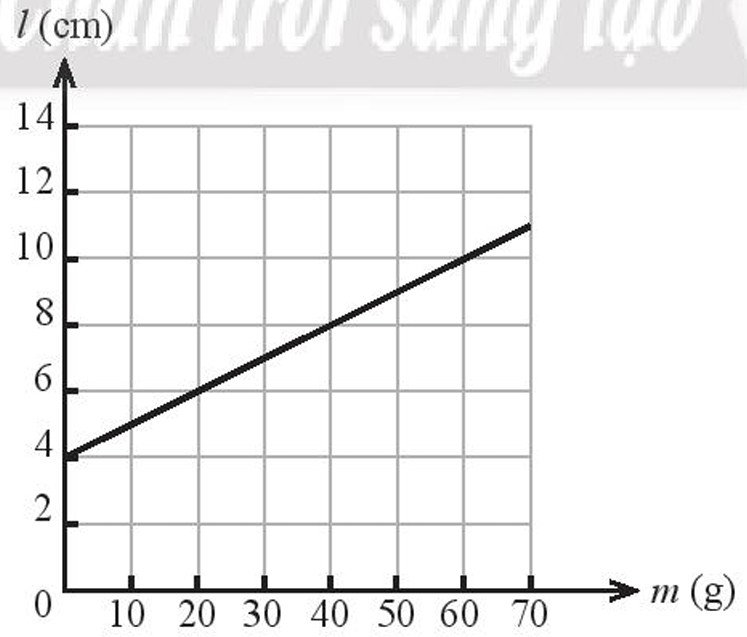
\includegraphics[scale=0.3]{figs/D10-ONTAPCUOINAM-2}}
	\loigiai{
		
	}
\end{ex}
% ===============================================================
\begin{ex}
	\immini{Một vật nặng có khối lượng bằng \SI{5}{\kilogram} được buộc vào một dây dài \SI{0.8}{\meter} và thả cho chuyển động trong mặt phẳng thẳng đứng như Hình bên. Khi qua vị trí cân bằng O, vật có tốc độ \SI{2.8}{\meter/
			\second}. Tính gia tốc hướng tâm và lực căng dây khi vật đi qua vị trí cân bằng O. Lấy $g=\SI{9.8}{\meter/\second^2}$.}{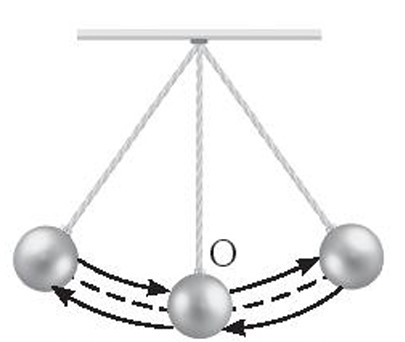
\includegraphics[scale=0.4]{figs/D10-ONTAPCUOINAM-1}}
	\loigiai{
		
	}
\end{ex}
% ===============================================================
\begin{ex}
	Một lò xo có độ cứng \SI{100}{\newton/\meter}, chiều dài tự nhiên \SI{36}{\centi\meter}, một đầu giữ cố định ở A, đầu kia gắn vào quả cầu khối lượng \SI{10}{\gram} có thể trượt không ma sát trên thanh nằm ngang. Thanh quay đều quanh trục $\Delta$ thẳng đứng với tốc độ 360 vòng/phút. Lấy $\pi^2=10$. Tính độ dãn của lò xo.
	\loigiai{
		
	}
\end{ex}
% ===============================================================
\begin{ex}
	Một ô tô tải kéo một ô tô con có khối lượng 2 tấn và chạy nhanh dần đều, sau \SI{50}{\second} đi được \SI{400}{\meter}. Khi đó dây cáp nối hai ô tô dãn ra một đoạn bao nhiêu trong trường hợp dây cáp song song mặt đất. Cho biết độ cứng của dây cáp là $k=\SI{2E6}{\newton/\meter}$ và bỏ qua mọi ma sát cùng khối lượng của dây cáp.
	\loigiai{
		
	}
\end{ex}
% ===============================================================
\begin{ex}
	\immini{Trong công viên giải trí, Bình An đang tham gia trò chơi "phòng không đáy". Trò chơi được vận hành như sau: người chơi bước vào căn phòng hình trụ bán kính \SI{3.0}{\meter}, căn phòng được cho quay đều với tốc độ \SI{5.0}{\radian/\second} như hình minh họa bên. Sau đó, sàn của căn phòng hạ xuống, để lại những người chơi tựa trên tường theo tư thế thẳng đứng. Xác định hệ số ma sát tối thiểu giữa quần áo của người chơi và bức tường để người không bị trượt xuống. Lấy gia tốc trọng trường $g=\SI{9.8}{\meter/\second^2}$.}{\vspace{-0.75cm}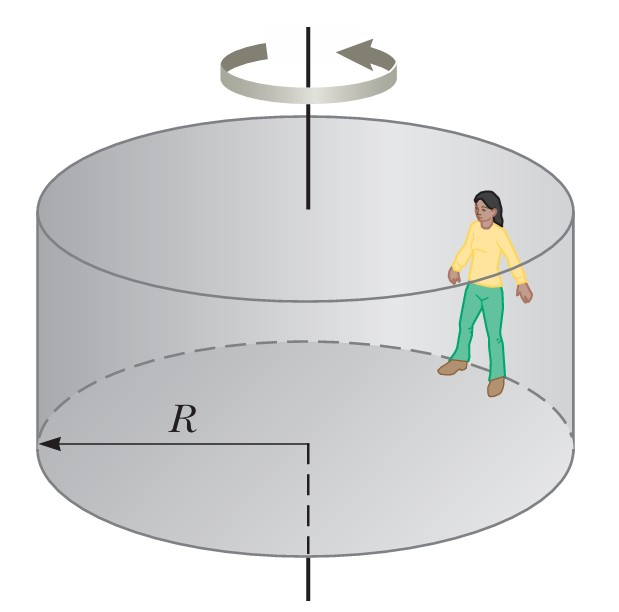
\includegraphics[scale=0.35]{figs/D10-ONTAPCUOINAM-3}}
	\loigiai{
		
	}
\end{ex}
\begin{center}
	\textbf{--- HẾT ---}
\end{center}